%% A simple template for a term report using the Hagenberg setup 
%% based on the standard LaTeX 'report' class

%%% Magic comments for setting the correct parameters in compatible IDEs
% !TeX encoding = utf8
% !TeX program = pdflatex 
% !TeX spellcheck = en_US
% !BIB program = biber

\RequirePackage[utf8]{inputenc} % Remove when using lualatex or xelatex!
\RequirePackage{hgbpdfa}        % Creates a PDF/A-2b compliant document

\documentclass[english,notitlepage,smartquotes]{hgbreport}
% Supported options in [..]:
%    Main language: 'german' (default), 'english'
%    Conversion to typographic quotation marks: 'smartquotes'
%    Use APA citation style: 'apa'
%    Do not create a separate title page: 'notitlepage'
%    Page layout: 'oneside' (single-sided, default), 'twoside' (double-sided)
%%%-----------------------------------------------------------------------------

\graphicspath{{images/}}  % Location of images and graphics
\bibliography{references} % Biblatex bibliography file (references.bib)
% theorems, definitions, remarks etc.
\usepackage{amsthm}

\theoremstyle{definition}
\newtheorem{definition}{Definition}

\theoremstyle{definition}
\newtheorem{problem}{Problem}

\theoremstyle{remark}
\newtheorem*{remark}{Remark}

\theoremstyle{definition}
\newtheorem{example}{Example}

\theoremstyle{plain}
\newtheorem{theorem}{Theorem}[chapter]
\newtheorem{corollary}{Corollary}[theorem]
\newtheorem{lemma}{Lemma}[chapter]
\newtheorem{mini-theorem}{Mini-theorem}
\renewcommand\qedsymbol{$\blacksquare$}
% theorems, definitions, remarks etc.
% the "reflection" box
\usepackage[framemethod=tikz]{mdframed}
\theoremstyle{definition}
\newtheorem{reflection}{Reflection}
\mdfdefinestyle{reflectionbox}{
  innertopmargin=\topskip,
  roundcorner=5pt,
  linecolor=cyan,
  backgroundcolor=cyan!20,
}
\surroundwithmdframed[style=reflectionbox]{reflection}
% the "reflection" box

% long table
\usepackage{longtable}
% long table

% for algorithm description
\usepackage{algorithm}
\usepackage{algpseudocodex}
% for algorithm description
% for images etc.
\usepackage{tikz}
\newcommand*\circled[1]{\tikz[baseline=(char.base)]{
    \node[shape=circle,draw=red,inner sep=2pt] (char) {#1};}}
\newcommand*\fillcircled[2]{\tikz[baseline=(char.base)]{
    \node[shape=circle,fill=#2,draw=red,inner sep=2pt] (char) {#1};}}
% for images etc.
% color names
\usepackage[pdftex,dvipsnames]{xcolor}
% color names
% Big starting letters
\usepackage{lettrine}
% Big starting letters
% cancel terms
\usepackage{cancel}
% cancel terms

% sidebar environment https://tex.stackexchange.com/a/735167/64425
\usepackage[most]{tcolorbox}

\newtcolorbox{sidebar}{
  breakable,
  enhanced,
  frame hidden,
  interior hidden,
  size=minimal,
  left skip=8pt,
  borderline west={1pt}{-5pt}{gray}
}
% sidebar environment https://tex.stackexchange.com/a/735167/64425

% 
\usepackage{parskip}% http://ctan.org/pkg/parskip
%
% todonotes
\usepackage{xargs}                      % Use more than one optional parameter in a new commands
\usepackage[colorinlistoftodos,prependcaption,textsize=tiny]{todonotes}
\newcommandx{\tbd}[2][1=]{\todo[linecolor=orange,backgroundcolor=orange!25,bordercolor=magenta,#1]{#2}}
\newcommandx{\doubt}[2][1=]{\todo[linecolor=red,backgroundcolor=red!25,bordercolor=black,#1]{#2}}
% todonotes
% get rid of ugly borders
\hypersetup{
    colorlinks,
    linkcolor={magenta!50!black},
    citecolor={blue!50!black},
    urlcolor={blue!80!black}
}
% get rid of ugly borders

% some commands, mainly for local use
% list of theorems
\usepackage{thmtools}
% list of theorems
% label list items
\usepackage{enumitem}
% label list items
% Place figures exactly where you mean to
%https://tex.stackexchange.com/a/8633/64425
\usepackage{float}
% Place figures exactly where you mean to
% failed proof
\newcommand{\bogusproof}{\textcolor{red}{\Huge\bf ?}}
% failed proof
% big O https://tex.stackexchange.com/a/354690/64425
%\usepackage{fourier}
%DeclareRobustCommand{\bigO}{%
% \text{\usefont{OMS}{cmsy}{m}{n}O}%
%
% big O https://tex.stackexchange.com/a/354690/64425
% some commands, mainly for local use
%%%-----------------------------------------------------------------------------
\begin{document}
%%%-----------------------------------------------------------------------------
\author{Kedar Mhaswade}                    % Your name
\title{The Art and Theory of Dynamic Programming by Stuart Dreyfus and Averill Law:\\ % Name of the course or project
			Notes and Problem Solutions}	                 % or "Project Report"
\date{09 July 2025}

%%%-----------------------------------------------------------------------------
\maketitle
%%%-----------------------------------------------------------------------------
\begin{abstract}\noindent

\bigskip
\noindent
% Use the abstract to provide a short summary of the document's contents.
\lettrine[lines=3]{T}{his} is an objective, yet personal, narrative of the author's odyssey in the enchanted land of dynamic programming. It contains his notes and solutions to problems from Professor Stuart Dreyfus and Professor Averill Law's \cite{DreyfusLaw1977} \textit{The Art and Theory of Dynamic Programming}.


I like to write. I don't have an established audience, but that does not deter me from writing. However, I have often wondered why I should carefully typeset my mathematical writing using a comprehensive system like \LaTeX. First, my mathematical writing is not `research' yet, but mainly problem-solving (which does involve at least some dogged pursuit, if not research). Second, I love writing by hand! 
\begin{figure}[!h]
\begin{center}
\caption{Handwriting is fun!}
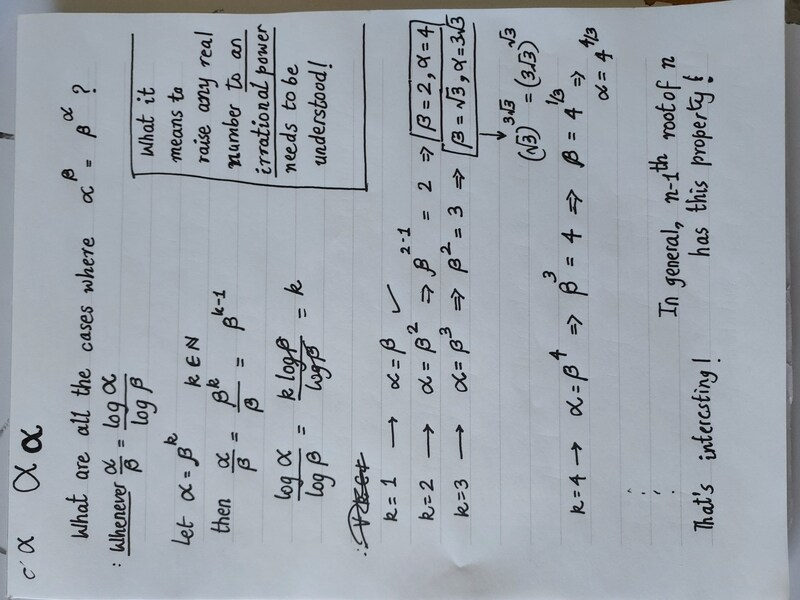
\includegraphics[width=.345\textwidth,angle=-90]{loving-to-write-by-hand-small}
\end{center}
\end{figure}

Freehand writing on a good paper with a good pen is fun. It's quick. It's rewarding.

Typesetting is, on the other hand, time-consuming and feels like \textit{Yak-shaving} \cite{Yak-shaving}. However, all good life is controlled Yak-shaving. When I typeset {\LaTeX} documents, I tend to minimize Yak-shaving and focus on having a conversation with myself. I suspect that I understand the subject matter better that way. I like the following quote in this regard:

\begin{sidebar}
I write because I don't know what I think unless I read what I say. -- Flannery O'Connor
\end{sidebar}

Of course, you cannot begin solving problems on a computer. A pencil and papers are must. In this respect, typesetting is favoring form (or sophistication) over content. We strive to present beautifully what we have thought well but scribbled hastily. Fortunately, I don't mind taking the time to do that; it at least keeps me busy fine-tuning my thoughts. It sometimes even helps to find flaws.

However, the biggest advantage of typesetting my writing is keeping a record of beautifully typeset account of something, anything. If I could ever make a case to study under a stalwart like Professor Yaser Abu-Mostafa (\url{https://work.caltech.edu/}), or Professor Avrim Blum (\url{https://home.ttic.edu/~avrim/}), perhaps I can demonstrate what I have done in my scarce free time.

I have gone back and forth between handwritten pages and typeset manuscripts. However, I am resorting to typesetting for this work despite the overhead incurred. I hope I follow through. It's one thing to be motivated but another to be determined and disciplined.

Perhaps a picture (Figure [\ref{fig:mindmap}]) can explain better than words how I started reading this book. 

\begin{figure}[!h]
\begin{center}
\caption{A July 2025 Mindmap}
\label{fig:mindmap}
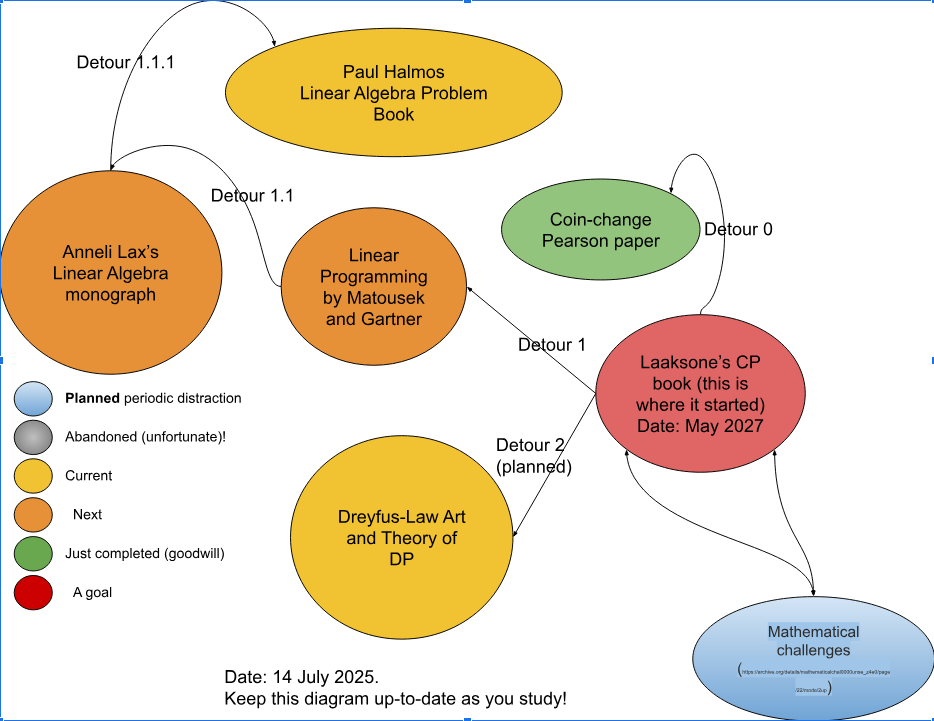
\includegraphics[width=.5\textwidth]{july-2025-mindmap}
\end{center}
\end{figure}

I will avoid answering ``Why Dreyfus-Law's Dynamic Programming\footnote{We'll affectionately call it DP in the following text} book''? It suffices to say that DP has been an exciting optimization technique that I hadn't been able to spend time on till now and that I wanted to correct that mistake by learning from a master\footnote{Prof. Dreyfus learned DP (and later co-developed it) from none other than its inventor, the influential and versatile mathematician, Dr. Richard Bellman}. Dreyfus teaches effectively in this book. His style is simple. 

This is one of the most readable, no-fluff, and comprehensive treatments of a challenging subject. Here is a sample of their style (which is very different from that of, say, Paul Halmos or Martin Gardner). One cannot \emph{not} be motivated to solve problems on his own and try to master the technique after reading something like this (emphasis mine):

\begin{sidebar}
It is our conviction, based on considerable experience teaching the subject, that the art of formulating and solving problems using DP can be learned only through \emph{active participation} by the 
student. 

\emph{No amount of passive listening to lectures or of reading text material prepares the student to formulate and solve novel problems}. The student must first discover, by experience, that proper formulation is not 
quite as trivial as it appears when reading a textbook solution. Then, by considerable practice with solving problems on his own, he will acquire the feel for the subject that ultimately renders proper formulation easy and natural. 

\emph{For this reason, this book contains a large number of instructional problems, carefully chosen to allow the student to acquire the art that we seek to convey. \textbf{The student must do these problems on his own.}}

Solutions are given in the back of the book because the reader needs\footnote{Many good problem-solving books stress this point} feedback on the correctness of his procedures in order to learn, but any student who reads the solution before seriously attempting the problem does so at this own peril\footnote{I have a personal ethic: Only check the solutions to the problems I was able to solve on my own. Check the solutions to the problems I couldn't solve in a reasonable amount of time after following the ``R. L. Moore'' procedure''}. 

He will almost certainly regret this passivity when faced with an examination or when confronted with real-world problems. We have seen countless students who have clearly understood and can religiously repeat our lectures on the DP solution of specific problems fail utterly on midterm examinations asking that the same techniques and ideas be used on similar, but different, problems. Surprised, and humbled, 
by this experience, the same students often then begin to take seriously our admonition to do homework problems and do not just read the solution and think ``of course that is how to do them,'' and many have written perfect final exams. 

\textbf{Why dynamic programming is more art than science we do not know. }

\emph{We suspect that part of the problem is that students do not expect to be called upon to use common sense in advanced mathematical courses and, furthermore, have very little practice or experience with common sense in this context. But common sense, not mathematical manipulation, is what it takes to be successful in a course in dynamic programming.}

While the preceding remarks are primarily addressed to the reader, the following comments on the organization and use of this text are mainly for the teacher. A certain amount of jargon is used in dynamic programming to express concepts that, while simple, come only from experience. Since we plan to tell the student this jargon only after he has experienced the concept, we believe that it is pointless and hopeless to tell the student, in advance and in a meaningful way, what the text will teach, how it is organized, etc. 

\emph{Our primary goal is to convey, by examples, the art of formulating the solution of problems in terms of the dynamic programming recurrence relations.}

The reader must learn how to identify the appropriate state and stage variables, and how to define and characterize the optimal value function. Corollary to this objective is reader evaluation of the feasibility and computational magnitude of the solution, based on the recurrence relation. Secondarily, we want to show how dynamic programming can be used analytically to establish the structure of the optimal solution, or conditions necessarily satisfied by the optimal solution, \emph{both for their own interest and as means of reducing computation}. Finally, we shall present a few special techniques that have proved useful on certain classes of problems. 
\end{sidebar}

I hope I can painstakingly (and gleefully at the same time) solve a number of problems from this book, and understand at least some of DP. Solutions in this text are mine. I have also felt free to think aloud, write willfully about questions that came to my mind as I solved the stated problems. That part of writing appears like ``personal reflections'':
\begin{reflection}
Problems come in various levels of difficulty. And, unless you are George Dantzig (who solved an open problem written on a blackboard assuming his instructor had given a homework assignment) or the like, you have to toil through them. Some you are able to solve quickly, perhaps because you are experiencing ``flow''\footnote{A highly focused mental state, defined and popularized by the psychologist Mihaly Csikszentmihalyi, conducive to productivity}, but many are challenging and you suffer (albeit purposefully) through them. They are distinct from exercises, which are also essential for fluency and emotional well-being, but are expected to be aimed at `practice' and easier to answer.

DP has been a particularly enigmatic optimization procedure for me. I have struggled to formulate an optimization problem as a DP problem. I am in awe of how DP magically provides an $O(n)$ solution to a problem for which conventional (brute force) approach can only provide an $O(n^3)$ or an $O(n^2)$ solution!

Is knowing DP technique \emph{thoroughly} in the age of AI needed? That's like asking, ``Is thinking for yourself necessary now that AI seems to take that over from us, for us?'' Since I enjoy learning DP just for the sake of it (gone are the days when I used to learn it superficially for clearing \emph{the Tech} interviews!), I don't care if AI will make my understanding irrelevant (it won't, because we want to make AI better and that can't happen just like that).

\end{reflection}

Feel free to skip them. 

As Dreyfus and Law urge us in his preface to this book, I have read their solutions too (readily for the problems I was able to finally solve--doing so is quite important--and begrudgingly for the problems I was not able to solve in quite some time). Solutions are an integral part of exposition. The $\blacksquare$ (QED symbol) appears wherever appropriate. Wherever desired, I have also reinterpreted their solutions (they appear under the heading \textbf{DL Solution}); understanding them will be certainly helpful. 

I am also embarking on a related extension of this personal project. This extension is mainly for my benefit, but it could be beneficial to others: \textbf{For at least some of the problems, I shall provide readable (beautiful?), correct, and efficient implementations in a programming language}\footnote{TODO: Provide some details}.
\end{abstract}

%%%-----------------------------------------------------------------------------
\tableofcontents
%%%-----------------------------------------------------------------------------

\chapter{Elementary Path Problems}

Dynamic programming is an \emph{optimization procedure} that is \emph{particularly applicable to problems requiring a sequence of interrelated decisions}. Each \emph{decision} transforms the current situation into a \emph{new situation}. 

\textbf{A sequence of decisions, which in turn yields a sequence of situations, is sought that maximizes (or minimizes) some measure of value.}

The value of a sequence of decisions is generally equal to the sum of the values of the individual decisions and situations in the sequence.

Here is an elementary, but instructive, motivating example (problem).


Consider a small and orderly, if somewhat unrealistic, city road network shown in Figure [\ref{fig:cityroads}]. The streets are all one-way and the numbers shown on the map's streets represent the \emph{effort} (that represents the idea of a `resource' in Economics) required to traverse the associated streets. 
\begin{figure}[!h]
\begin{center}
\caption{A City Road Network}
\label{fig:cityroads}
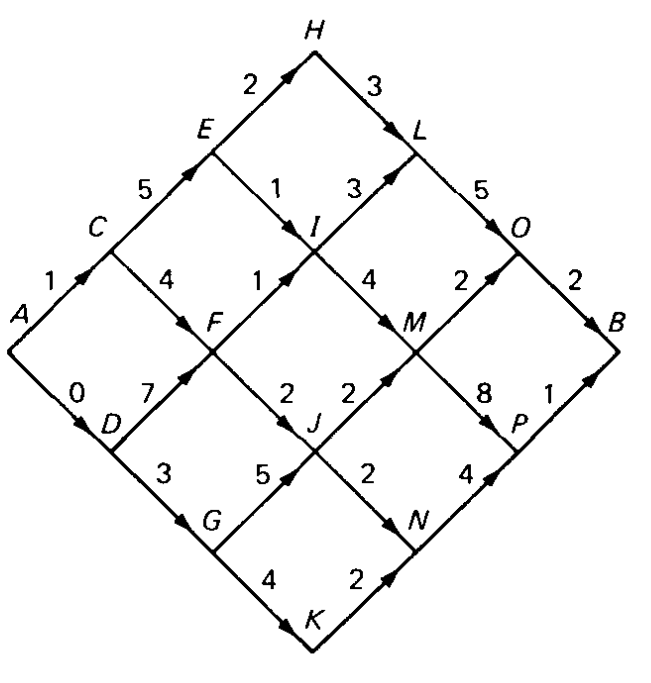
\includegraphics[width=.345\textwidth]{elem-path-problem-1}
\end{center}
\end{figure}

Which path will you take from A to B so as to \emph{minimize the total effort}?

\begin{reflection}
One gets a sense of optimization in this problem statement. If you are a `techie', then you can already brand this problem as a ``DP Problem''. Since this is a canonical DP problem (appearing at the outset in a book on DP), this suspicion is appropriate. The feeling that DP can solve almost any optimization problem stems not from a sound understanding of the technique but from a weird expectation where a problem is introduced so as to invite a brute-force solution that can always be improved upon by applying DP.

But first, everyone should attempt to correctly solve a problem somehow, verify the solution, and then optimize it by identifying the sources of inefficiencies incurred in a previous solution (that is now correct, but inefficient). That is the process of any computational optimization.
\end{reflection}


This is a small network displaying regularity and a visual inspection tells us that at every point (except of course B) or vertex starting from A, one can only make one of two choices for an arc (or block) to take: northeast or southeast. If it were a large network, we had to know a priori that it follows some structure (without resorting to inspection, which would be too time-consuming). 

A path between any two vertices (the latter, called the \emph{target}, being to the east of the former, called the \emph{source}) is a sequence of arcs. For example, one path from D to M is DF-FJ-JM. The length of a path is the number of arcs in it regardless of the effort required to take an arc. Thus, the length of the path DF-FJ-JM is 3.

The total effort of a path is the sum of the efforts for its arcs. Thus, the total effort of the path DF-FJ-JM from D to M is $7+2+2=11$. The path with the least total effort is the best path. 

How many paths are there from a given source to a given target, assuming the target is to the east of the source (otherwise there are no paths)?   

That tricky question concerns `counting' and we resort to combinatorial techniques to answer it in general. 

We soon realize that the lengths of all the paths from a given source to a given target must be equal\footnote{TODO: Need a rigorous proof of this}. If a southeast arc of a path is denoted by SE and northeast arc by NE, we have an `n-string' like SE-NE-NE-SE-\dots each segment of which is either `SE' or `NE'. Thus, if a path between any two vertices comprises $s$ southeast arcs and $n$ northeast arcs, all paths between those vertices do. Therefore, the total number of paths then is the number of ways you reach the target is the same as the total number of ways you can choose either $s$ southeast arcs or $n$ northeast arcs while taking a total of $s+n$ arcs\footnote{Alternatively, one can say that the number of paths from A to J equals the number of paths from A to F plus the number of paths from A to G because each of those paths (and no other) can reach J}. This number is ${s+n\choose s}={s+n\choose n}$.

The total number of paths from A to B are the total number of ways to choose three southeast or three southwest arcs in a path length of 6 arcs that is ${6 \choose 3}=\frac{6\cdot 5\cdot 4}{3\cdot 2\cdot 1}=20$. 

Now, to find the \emph{best} path, one enumerates each of these 20 paths and compares the effort required for each one. The length of each path from A to B is 6 and calculating the effort required results in 5 additions. The total number of additions equals $5\times 20=100$. The total number of comparisons is 19. After all these computations, we have the best path. This is the brute-force solution.

This `enumerative' solution that examines every path from A to B and determines the best path is perhaps straightforward to think of\footnote{Implementing it correctly and succinctly as a computer program is still a challenge}. 

Can we do better?
\begin{reflection}
This question often baffles me. What makes us suspect a `better' solution to a computational problem? 

I guess an experience in dealing with problem statements helps. Many computational problems are like word problems in elementary school algebra. If we are aware of theoretical limits of certain operations (for example, the ``information theoretic limit'' on sorting a random list of integers is $O(n\log n)$--it's futile to try to find a better general solution for sorting), then we can look for any information (usually hidden) in the specification of the problem.

I have often wondered if there is an algorithm mechanically following which one can improve a solution (to a computational problem). I am not sure. That's why programming is sometimes called art (even in the age of AI, albeit by a diminishing number of people).

Closely reading the problem statement, looking for cues to improve a solution, arguing logically, patiently nurturing imagination (or common sense) while being guided by knowledge may help.

This endeavor is in the spirit of problem-solving as elucidated by the phenomenal writings of maestros like P\'olya (cf. \cite{Polya2004}) and Gardner (cf. \cite{GardnerSciAmColumns}) among several others.

One aspect of the ``optimization problems'' like this one is that \emph{some} solution is not enough. In the spirit of computation, we are asked to compute what is computable as efficiently as possible. Any \emph{needless computation} must be avoided. This requirement makes it trickier.

Some may argue, ``Computers are becoming faster and faster, why do you need to optimize?'' But then we may counter, ``Why do you need computers at all?''

Optimization is key. For \emph{small} problems suboptimal solutions are perhaps acceptable. But for large problems, suboptimal (and slow) solutions may even be worse than wrong (but quick) solutions. Is such obsessive approach to efficiency, productivity, optimization necessary in the age where human attention span is ever becoming shorter, computer hardware (apparently) cheaper and abundant, and computer programming as a human skill obsolete? 

That's a matter of perspective. In our view, learning the theory and techniques of optimal algorithms is an essential, if advanced, part of computer programming. Fortunately, dynamic programming is a well-established technique whose accurate application to a problem can bring you joy even if you are not solving a ``production issue'' or appearing for a technical interview. The actual `in-silico' performance of a solution to a computational problem is a complicated business, but, in keeping with Occam's Razor, we'll get the biggest bang for the performance buck with accurate modeling, sound theory, and clutter-free implementation.

``Beauty is the first test: there is no permanent place in the world for ugly mathematics.'', thus wrote the famous mathematician G. H. Hardy in \cite{Hardy1940}. We contend that a certain beauty, an elegance oozes through an optimal solution. 

Of course, DP is a \emph{technique} to eliminate inefficiencies in brute-force solutions. It does not change the ``intractability characteristics'' of computational problems. Intractability is a property of truly difficult problems of which there is no dearth. DP is not a panacea for solving such hard problems. Rather it is an effective way to implement practical solutions to difficult problems. These solutions are often realized through computer programs. As a result of this, the ``formulation of a DP solution'' to some problem is often called its ``DP algorithm''.

The DP solution to this problem described in the book is highly readable. We are going to skip that here because reading it from the book (rather than these notes) is the best one can do. We will only reproduce a gist of the discussion here:
\begin{sidebar}
One of the two \emph{key ideas} of DP has already made its innocuous appearance. This is the observation that only the efforts along the best paths from C and D to B are relevant to the above computation, and the efforts along the nine\footnote{There are ${5\choose 2}=10$ paths from each of C and D to B; only one of those is optimal} inferior paths from each of C and D to B need never be computed. This observation is called the Principle of Optimality and is stated as follows:
\begin{definition}[Principle of Optimality]
\label{def:poopt}
The best path from A to B (with 0 or more vertices between them) has this property that, \emph{whatever the initial decision at A}, the remaining path to B, starting from the next vertex after A, must be the best path from that vertex to B.
\end{definition}

This is an illuminating definition. It is almost an axiom, a self-evident principle: Of all the paths from A to B, how can A--X--Y--Z--B be the best, unless X--Y--Z--B is the best of all paths from X to B?

The second idea is similar to the base case of recursion. We start at a vertex that is closest to our target, B, and readily compute the `constant-time' boundary conditions. Then we work backward, further and further away from it and as we do that we only compute the lengths of the best (partial) paths in accordance with the Principle of Optimality [\ref{def:poopt}]. 

The goal is to set up recurrence relations and solve them. Paraphrasing the following from the book:

\textbf{It may surprise the reader to hear that there are no further key ideas in dynamic programming}. \emph{Naturally, there are special tricks for special problems, and various uses (both analytical and computational) of the foregoing two ideas, but the remainder of the book and of the subject is concerned only with how and when to use these ideas and not with new principles or profound insights. What is common to all dynamic programming procedures is exactly what we have applied to our example: first, the recognition that a given “whole problem” can be solved if the values of the best solutions of certain subproblems can be determined (the principle of optimality [\ref{def:poopt}]); and secondly, the realization that if one starts at or near the end of the ``whole problem,'' the subproblems are so simple as to have trivial solutions (like the recursive base cases).}
\end{sidebar}
\end{reflection}

Some terminology is indispensable. We'll solve problems with this terminology in mind.
\begin{table}[h!]
\centering
\begin{tabular}{l|l|l}
Name&Symbol&Meaning\\
\hline
Principle of Optimality & -- & \multicolumn{1}{p{6cm}}{See Definition [\ref{def:poopt}].}\\
Optimal Value Function & $S$ & \multicolumn{1}{p{6cm}}{The \emph{rule} that assigns values to various subproblems. For example, the total effort for the optimal path is a real number like $15.8$.}\\
Optimal Policy Function & $P$ & \multicolumn{1}{p{6cm}}{The \emph{rule} that associates the best first decision with each subproblem. For example, the optimal path (as a sequence of vertices) is A--X--Y--Z--B.}\\
Argument(s) (to $S,P$) & $x,y,\dots$ & \multicolumn{1}{p{6cm}}{Similar to classical function's arguments; giving actual values to arguments captures specific subproblems.}\\
\multicolumn{1}{p{4cm}|}{\raggedright Recurrence Relations (or Recurrences)}& \multicolumn{1}{|p{3cm}|}{\raggedright E.g. $S(x)=min(2+S(y),3+S(z))$} & \multicolumn{1}{p{6cm}}{The set of formulas (equations) involving values of $S$ \textit{recurrently}. Some of the recurrences are associated with the ``whole problem''. Our goal is to formulate and solve the whole-problem recurrence relations according to [\ref{def:poopt}].}\\
Boundary Conditions on $S$ & $S(a),S(b),\dots$ & \multicolumn{1}{p{6cm}}{Certain values of $S$ that are assumed obvious from the problem statement and which require no computation (requiring $O(1)$ computational cost). We typically work backward from them.}\\
Stage&--&\multicolumn{1}{p{6cm}}{Typically, but not necessarily, a path vertex where a decision needs to be made, multiple choices may exist, and making any choice incurs computational cost in terms of elementary operations like adding or comparing numbers. Total computational cost is the sum of costs incurred at stages. Sometimes stage may refer to arcs in a network path.}\\
\hline
\end{tabular}
\caption{Our Terminology}
\label{tab:dpterms}
\end{table}

Here is the essence of DP as it appears in the book (Pg. 7):

\hrulefill

In the exercises assigned during this and subsequent chapters, when we use a phrase such as, ``Give the dynamic-programming formulation of this problem,'' we shall mean: 
\begin{enumerate}
\item Define the appropriate optimal value function, including both a specific definition of its arguments and the meaning of the value of the function (e.g. $S(x,y)=$ The \textit{value} of the best path connecting the vertex $(x,y)$ (the source) with the vertex $(6,0)$ (the target))
\item Write the appropriate recurrence relations (e.g. $S(x,y)=\min(f(x,y) + S(x+1,y+1), g(x,y)+S(x+1,y-1), h(x,y)+S(x-1,y+1),\dots$); the book uses a nonstandard, matrix-like notation for the $\min$ function that looks better, we'll sometimes use that)
\item Note the appropriate boundary conditions (e.g. $S(6,0)=0$) and solve the recurrences
\end{enumerate}
\hrulefill


And, lest we forget, here is the stark reminder again:

\hrulefill

\textbf{As we emphasized in the Preface, the art of dynamic-programming formulation can be mastered only through practice, and it is absolutely essential that the reader attempt almost all of the assigned problems.  Furthermore, the student should understand the correct solution given in the back of this book before continuing.}

\hrulefill

(As a personal policy, we'll readily see solutions to the problems that we have solved confidently, and rather \emph{begrudgingly} of those that we couldn't solve even after working hard.)


\begin{problem}[A Line Target]
\begin{figure}[!h]
\centering
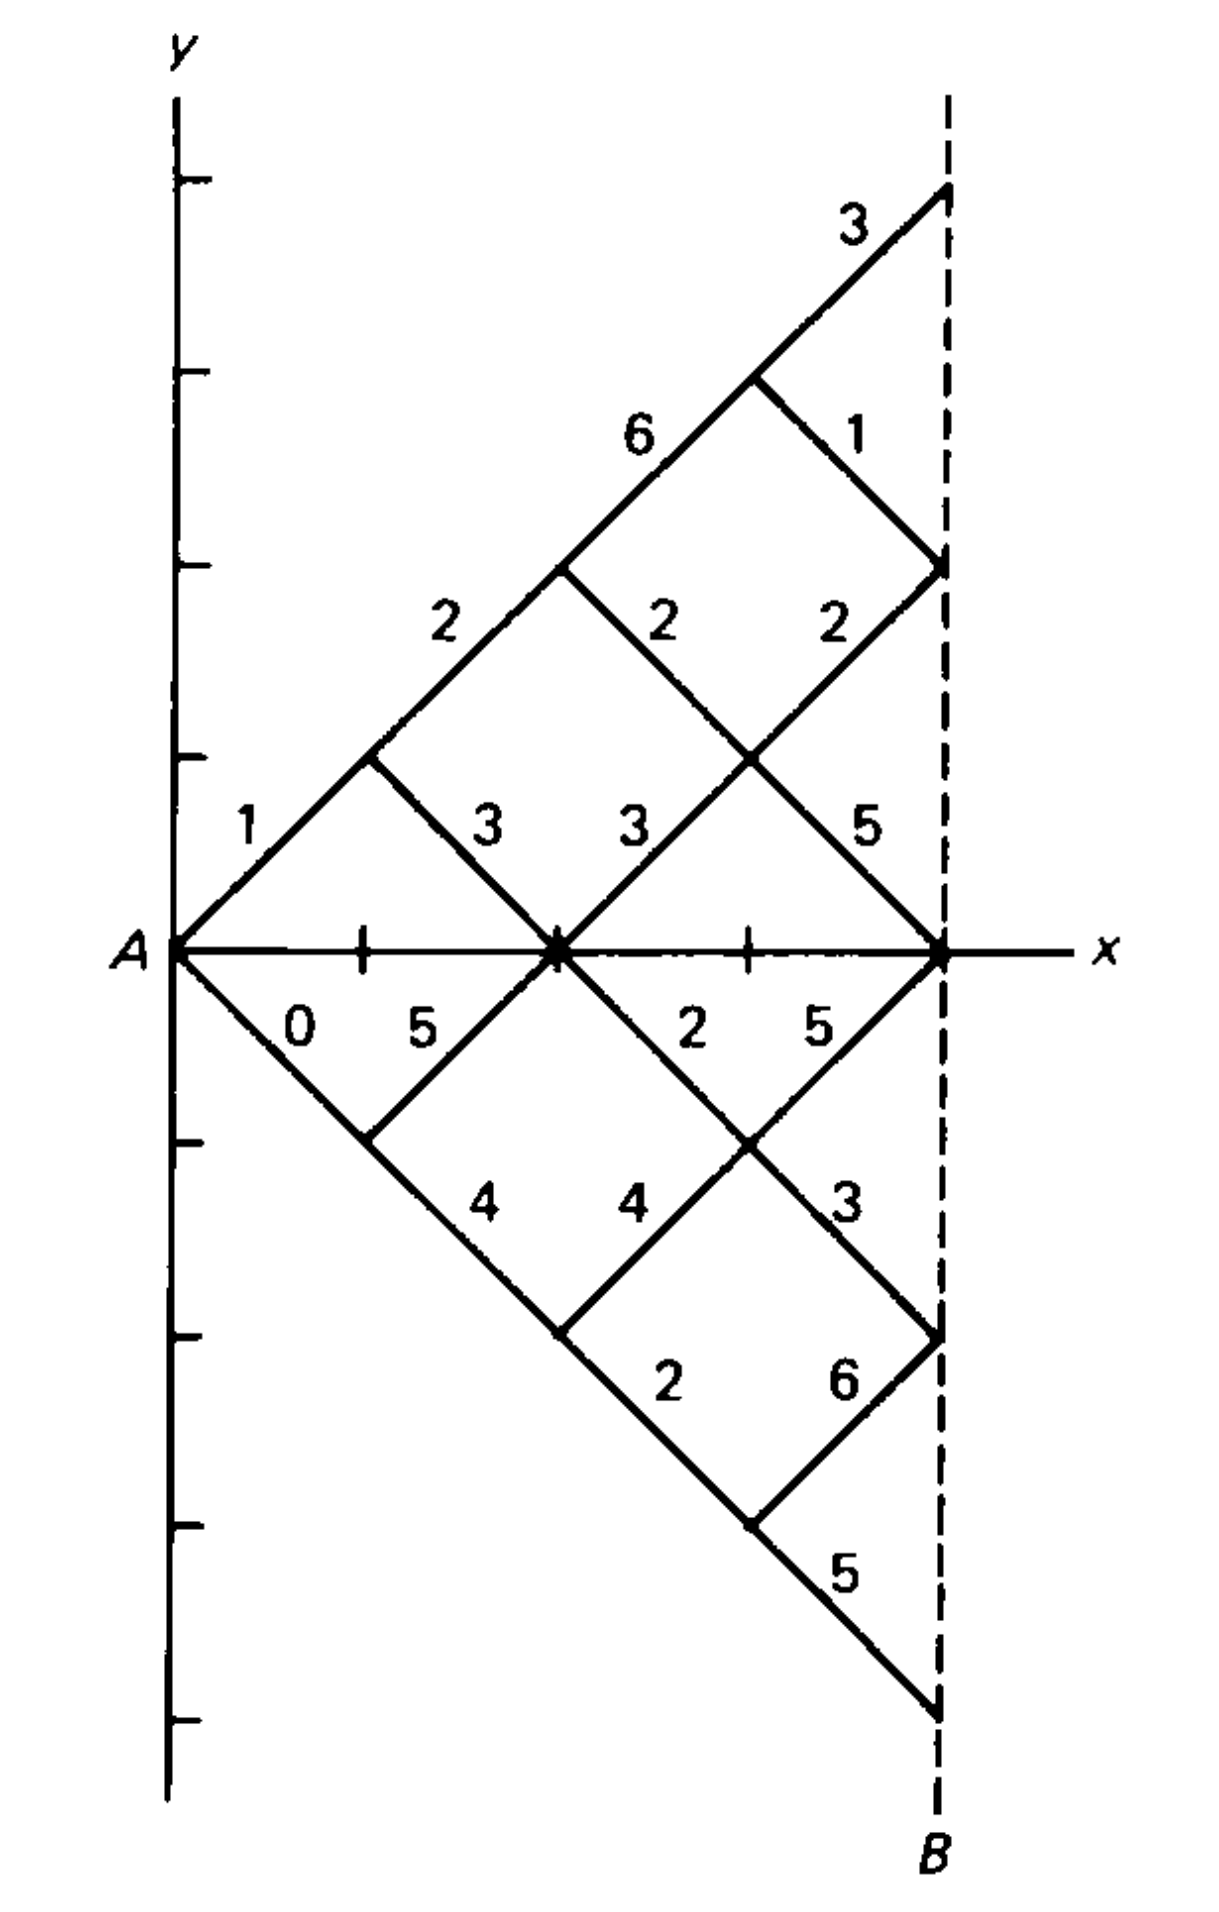
\includegraphics[width=.345\textwidth]{p11-pt-to-line}
\caption{Network for Problem [\ref{pr:1.1}]}
\label{fig:p1.1}
\end{figure}
On the network shown in Figure [\ref{fig:p1.1}]\footnote{TODO: Convert to TikZ}, we seek that path connecting A with any point on line B which minimizes the sum of the four arc numbers encountered along the path. (There are 16 admissible paths.) Give the dynamic-programming formulation of this problem.
\label{pr:1.1}
\end{problem}
\textbf{Solution}.

There are 16 admissible paths, each with 4 arcs. The brute-force solution will entail $16\times(4-1)=48$ additions and 15 comparisons to yield the best path. 

Can we do better?

\begin{reflection}
We observe that if we were already at \emph{any} of the five vertices $(4,4)$,$(4,2)$,$(4,0)$,$(4,-2)$, and $(4,-4)$, we would be done; no more effort is needed to reach our goal i.e. the line $x=4$. 

If, however, we knew the optimal efforts required to reach the line $x=3$, i.e., \emph{all} of the four vertices, $(3,3)$, $(3,1)$, $(3,-1)$, and $(3,-3)$, we could reach the line $x=4$ \emph{optimally} by doing $4\times2=8$ additions (yielding 8 numbers) and $8\div2=4$ comparisons.

Similarly, if we knew the optimal efforts required to reach the line $x=2$, i.e., \emph{all} of the three vertices, $(2,2)$, $(2,0)$, and $(2,-2)$, we could reach the line $x=3$ optimally in $3\times2=6$ more additions and 3 more comparisons.

Similarly, if we knew the optimal efforts required to reach the line $x=1$, i.e., both the vertices, $(1,1)$ and $(1,-1)$, we could reach the line $x=2$ in $2\times2=4$ more additions and 2 more comparisons.

Finally, if we do 2 more additions and 1 more comparison to reach the line $x=1$ optimally from A, we could find the optimal path from A to the line $x=4$ by doing 20 additions and 10 comparisons.

If an addition and a comparison is assumed equally expensive, this is about twice as efficient as the brute-force solution.

We have considered the Principle of Optimality and it seems like a DP formulation of the problem.
\end{reflection}

Consider Optimal Value Function and associated Optimal Policy Function:
\begin{equation}
\begin{aligned}
S(x,y)&=\text{ Value of the best path from the vertex $(x,y)$ to the line $x=4$}\\
P(x,y)&=[(x_1,y_1),(x_2,y_2),\dots,(x_n,y_n)] \\
\label{eq:p11ovf}
\end{aligned}
\end{equation}

(where $(x_i,y_i)$ are the vertices and $n$ is the length of the best path from $(x,y)$ to the line $x=4$)

We denote by $p(x,y)$ the parent vertex of the vertex $(x,y)$. In a path, if $(x_1,y_1)$ \emph{precedes} $(x_2,y_2)$, then $p(x_2,y_2)=(x_1,y_1)$. The source vertex of a path does not have a parent. It is possible that a vertex has multiple parents (because a vertex can appear on multiple paths).

Working through the network from vertex A to line B, we get the following recurrences:
\begingroup
\allowdisplaybreaks
\begin{equation}
\begin{aligned}
S(0,0) &=\min
  \begin{pmatrix}
  1+S(1,1) \\
  0+S(1,-1)
  \end{pmatrix}\\
S(1,1) &=\min
  \begin{pmatrix}
  2+S(2,2) \\
  3+S(2,0)
  \end{pmatrix}\\
S(1,-1) &=\min
  \begin{pmatrix}
  5+S(2,0) \\
  4+S(2,-2)
  \end{pmatrix}\\
S(2,2) &=\min
  \begin{pmatrix}
  6+S(3,3) \\
  2+S(3,1)
  \end{pmatrix}\\
S(2,0) &=\min
  \begin{pmatrix}
  3+S(3,1)\\
  2+S(3,-1)
  \end{pmatrix}\\
S(2,-2) &=\min
  \begin{pmatrix}
  4+S(3,-1)\\
  2+S(3,-3)
  \end{pmatrix}\\
S(3,3) &=\min
  \begin{pmatrix}
  3+S(4,4)\\
  1+S(4,2)
  \end{pmatrix}\\
S(3,1) &=\min
  \begin{pmatrix}
  2+S(4,2)\\
  5+S(4,0)
  \end{pmatrix}\\
S(3,-1) &=\min
  \begin{pmatrix}
  5+S(4,0)\\
  3+S(4,-2)
  \end{pmatrix}\\
S(3,-3) &=\min
  \begin{pmatrix}
  6+S(4,-2)\\
  5+S(4,-4)
  \end{pmatrix}\\
\end{aligned}
\label{eq:p11rr}
\end{equation}
\endgroup

Since the line $x=4$ can only be reached by reaching \emph{any} of the five vertices $(4,4)$,$(4,2)$,$(4,0)$,$(4,-2)$, and $(4,-4)$, we get the following boundary conditions:

\begin{equation}
\begin{aligned}
S(4,4) &= 0\\
S(4,2) &= 0\\
S(4,0) &= 0\\
S(4,-2) &= 0\\
S(4,-4) &= 0\\
\end{aligned}
\label{eq:p11bc}
\end{equation}

Solving equations [\ref{eq:p11rr}] using the boundary conditions from equations [\ref{eq:p11bc}], we get:
\begin{equation}
\begin{aligned}
S(3,-3) &= 5\;\therefore p(4,-4)=(3,-3)\\
S(3,-1) &= 3\;\therefore p(4,-2)=(3,-1)\\
S(3,1) &= 2\;\therefore p(4,2)=(3,1)\\
S(3,3) &= 1\;\therefore p(4,2)=(3,3)\\
S(2,-2) &= \min(4+3,2+5)=7 \therefore p(3,-1)=(2,-2), p(3,-3)=(2,-2)\\
S(2,0) &= \min(3+2,2+3)=5\therefore p(3,-1)=(2,0), p(3,1)=(2,0)\\
S(2,2) &= \min(6+1,2+2)=4\therefore p(3,1)=(2,2)\\
S(1,-1) &= \min(5+5,4+7)=10\therefore p(2,0)=(1,-1)\\
S(1,1) &= \min(2+4,3+5)=6\therefore p(2,2)=(1,1)\\
\text{And, finally, } S(0,0) &=\min(1+6,0+10)=7\therefore p(1,1)=(0,0)
\end{aligned}
\label{eq:p11sol}
\end{equation}

Traversing the $p$'s in the other direction, we get the optimal path:
\[
P(0,0)=[(0,0),(1,1),(2,2),(3,1),(4,2)]
\]
\textbf{DL Solution}. The straightforward solution appears on Pg. 217 of the book. Our solution agrees with it. The textbook solution gives the best path $P(0,0)$ but does not give the \emph{value} $S(0,0)=7$ (of course, finding $S(0,0)$ is straightforward).

\begin{reflection}[Need to Implement DP Solutions as Computer Programs]
Once you know the technique, finding the correct answer is perhaps straightforward. It could even be boring. Indeed, like the great mathematician Gauss once said, ``It is not knowledge, but the act of learning, not the possession of but the act of getting there, which grants the greatest enjoyment''.

Solving the recurrences was fun, but we keep feeling that we may make some human error. We keep feeling that a computer should be taught to do this! Also, this network was small. Toiling through bigger networks by hand is even more error-prone. 

Therefore, I must write computer programs to solve these problems\dots
\label{ref:needtoprog}
\end{reflection}

\begin{reflection}

\textbf{Accurate modeling of the problem is crucial! And we know that all models are wrong, but some are useful.}

This problem could also be modeled as a mere extension of our motivating example (Figure [\ref{fig:cityroads}]). Since from that example we know how to go from a source vertex to a target vertex, we could calculate the best path from $(0,0)$ to $(4,4)$, and the best path from $(0,0)$ to $(4,2)$, and so on. That would yield us five different paths and five values for $S(0,0)$, the smallest of which is also the best path from $(0,0)$ to the line $x=4$! 

However, modeling it that way and calculating each path using DP would be like being penny wise and pound foolish.

I must admit that the thought of solving it this way did cross my mind\footnote{And, in fact, this is the brute-force solution}.
\end{reflection}

\begin{problem}[A Network with a Target Rebate]
Solve the above problem (Figure [\ref{fig:p1.1}]) using dynamic programming, with the additional specification that there is a rebate associated with each terminal point; ending at the point (4, 4) has a cost of $-2$ (i.e., 2 is subtracted from the path cost), (4, 2) $-1$, (4, 0) $-3$, $(4, -2)$ $-4$, and $(4, -4)$ $-3$.
\end{problem}
\begin{reflection}
Oh, this is the same problem with different boundary condition values; I need a computer program!

I believe I can create a framework for solving such two-dimensional network problems, but I'll wait to read further so that I can accommodate a good number of problems.

I will skip this problem for now \dots
\end{reflection}


\begin{figure}[!h]
\begin{center}
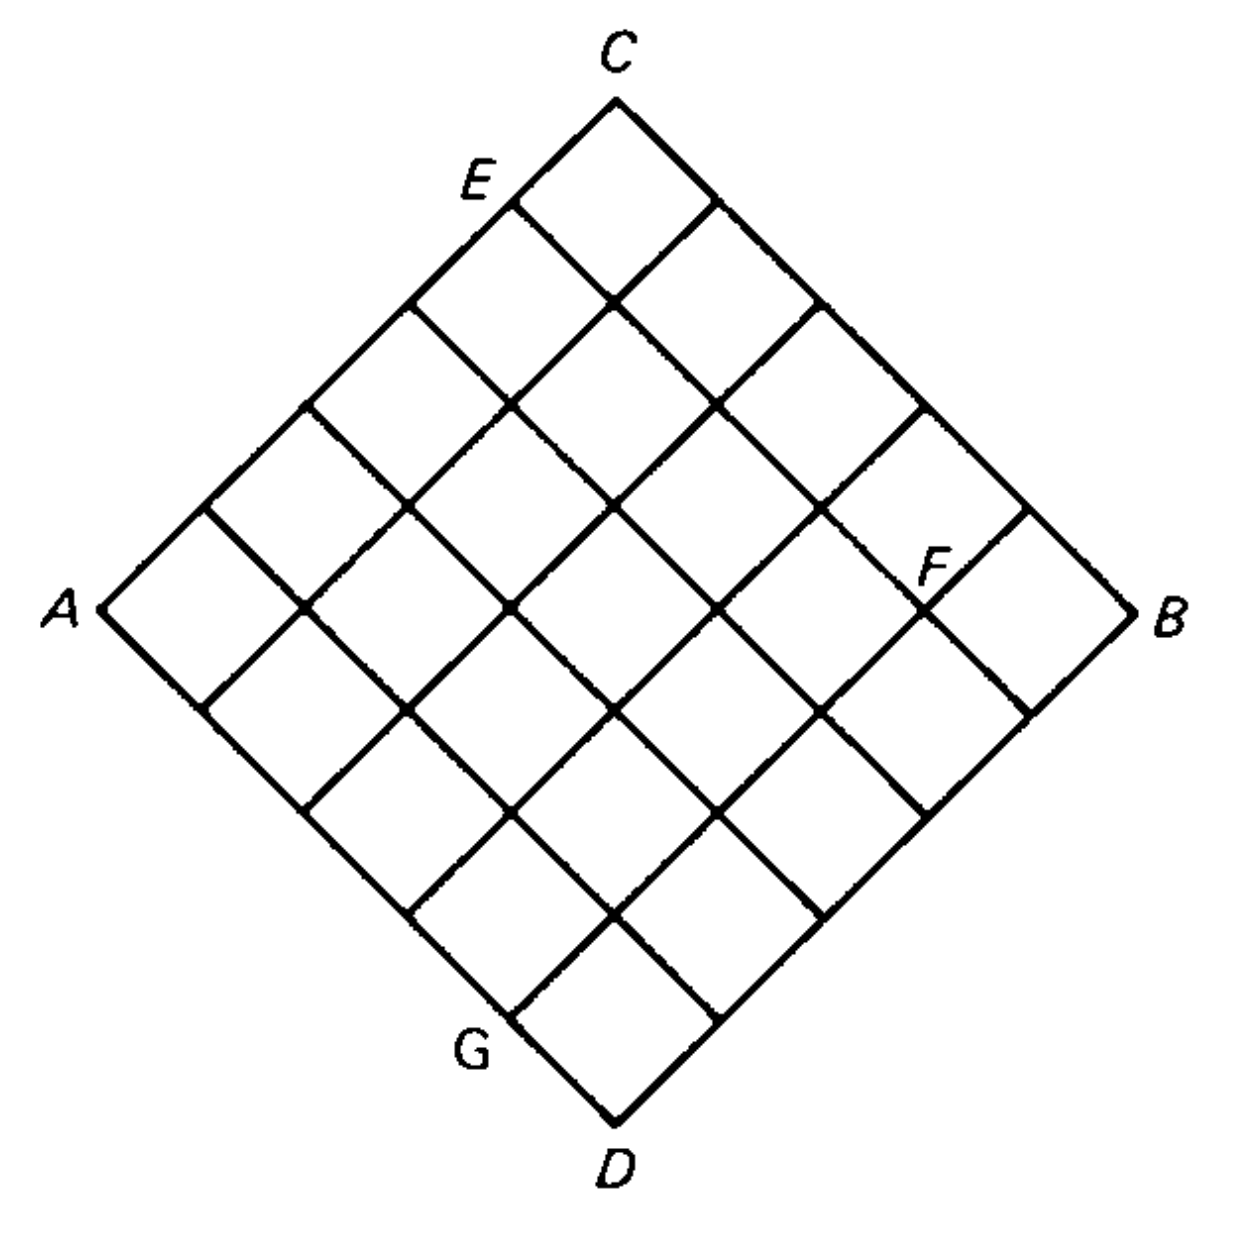
\includegraphics[width=.345\textwidth]{p14-n-stage-nenw-network}
\caption{A General N-stage NE-SE Network}
\label{fig:general-network}
\end{center}
\end{figure}


We now compare the brute-force solution with the DP solution in terms of computational efficiency: Can we quantify how much better the DP solution is than the brute-force solution in general for the network in Figure [\ref{fig:general-network}]?

Our endeavor is to make a fairly accurate approximation to the exact number of calculations. The exact number is not that important.

This is an N-stage network. Every path (optimal or not) has N arcs along which we need to make decisions. 

At $\frac{N}{2}$ vertices along the edge CB and at $\frac{N}{2}$ vertices along the edge DB we need only to add one number to a running total because there is a forced choice there. At B, there is no choice by default; once we reach B, we are done.

\begin{equation}
\begin{aligned}
\text{Number of Edge Additions}=\frac{N}{2}+\frac{N}{2}=N
\end{aligned}
\label{eq:numcaledge}
\end{equation}

All the vertices on and inside the square AGFE are equally expensive; we need to do two additions and one comparison at each vertex. There are $\frac{N}{2}\cdot\frac{N}{2}=\frac{N^2}{4}$ such vertices.

\begin{equation}
\begin{aligned}
\text{Number of Core Additions}&=2\times\frac{N}{2}\times\frac{N}{2}=\frac{N^2}{2}\\
\text{Number of Core Comparisons}&=\frac{N}{2}\times\frac{N}{2}=\frac{N^2}{4}
\end{aligned}
\label{eq:numcalcore}
\end{equation}

From equations [\ref{eq:numcaledge}] and [\ref{eq:numcalcore}], we have 
\begin{equation}
\begin{aligned}
\text{Total Number of Additions}&=\frac{N^2}{2}+N\\
\text{Total Number of Comparisons}&=\frac{N^2}{4}\\
\therefore \text{Total Cost (Additions+Comparisons)}&=O(N^2)
\end{aligned}
\label{eq:numcaltotal}
\end{equation}

Big-Oh notation is used to mathematically compare growth of functions. Equation [\ref{eq:numcaltotal}] implies that the cost of the optimal path in our network is a polynomial (quadratic) in the number of arcs in it. This is a helpful indicator.

Let's analyze the performance of the brute-force solution. In the network that has $N$ arcs, we must take $\frac{N}{2}$ north-easterly or north-westerly arcs. The total number of paths is then ${N \choose \frac{N}{2}}$ which is exponential in $N$. Each path must entail $N-1$ additions and the total cost is $O(N\cdot 2^{\frac{N}{2}})$. This solution is unacceptably slow for large values of $N$.

\hrulefill

\begin{problem}[Analyze the Line Target Network]
How many additions and how many comparisons are required in the DP solution and in the brute-force enumeration for an N-stage problem involving a network of the type shown in Figure [\ref{fig:p1.1}]? Evaluate your formulas for N = 20.
\end{problem}

\textbf{Solution}.

The DP solution revolves around the number of vertices in the network. Every line of $n$ vertices starting from the source vertex connects to a subsequent line that has $n$ vertices and one more. In an $N$-stage network, the target line has $N+1$ vertices at which no computation is needed. Thus, all the computations of the DP solution occur at all of the $1+2+3+\dots+N$ (`inner') vertices. At each vertex, we perform two additions and one comparison. Therefore, the DP solution needs $2\times(1+2+3+\dots+N)=N^2+N$ additions and $\frac{N(N+1)}{2}$ comparisons. For $N=20$, these are 420 and 210 respectively.

The brute-force solution is enumerative. The number of paths reaching every vertex in the network form the famous ``Pascal's Triangle''\footnote{We may use mathematical induction to prove it formally} along the vertical lines. Specifically, the number of `terminal' vertices in such $N$-stage network equals the sum of \emph{coefficients of the binomial}: $(a+b)^N$. This sum is $2^N$, because $\displaystyle\sum_{i=0}^{N}{N\choose i}=(1+1)^N=2^N$. Since the brute-force solution enumerates every path, requires $N-1$ additions for each, and finally $2^N-1$ comparisons, it needs $(N-1)\times2^{N}$ additions and $2^{N}-1$ comparisons in all. For $N=20$, these are 19,922,944 and 1,048,575 respectively!

\textbf{DL Solution}. Our solution agrees with theirs!

\hrulefill

In path-problems such as these, one can always look at the best path differently. Earlier, following the Definition [\ref{def:poopt}], we considered the implication that the best path A--X--Y--Z--B from A to B implies the best path X--Y--Z--B from X to B. That begs a question: If A--X--Y--Z--B is the best path from A to B, then isn't A--X--Y--Z the best path from A to Z?
\begin{definition}[Forward Variant of Principle of Optimality]
\label{def:pooptforward}
The best path from A to any vertex B has the property that whatever the vertex before B, call it C, the path must be the best path from A to C.
\end{definition}
Indeed, considering the contrapositive, if A--X--Y--Z is \emph{not} the best path from A to Z, then A--X--Y--Z--B is \emph{not} the best path from A to B, even if Z--B is the best path from Z to B.

With this definition, we can reformulate another variant of DP problems. In this formulation that we call the Forward Dynamic Programming, unlike the previous formulation which is called the Backward Dynamic Programming, $(x,y)$ is the target vertex and the source vertex is usually $(0,0)$:

\begin{equation}
\begin{aligned}
\text{Optimum Value Function}\\ 
S(x,y)&=\text{ Best-path Value Source to Target $(x,y)$}\\
\text{Optimum Policy Function}\\
P(x,y)&=[(x_1,y_1),(x_2,y_2),\dots,(x,y)] \\
\text{Recurrence Relations}\\
S(x,y)&=
\min\begin{pmatrix}
f(x-1,y-1)+S(x-1,y-1)\\
g(x-1,y-1)+S(x-1,y-1)\\
\dots
\end{pmatrix}\\
\text{Boundary Conditions (at Source)}\\
S(0,0)&=0
\label{eq:fwddp1}
\end{aligned}
\end{equation}

Let's compare the Optimal Value Functions of the two \textbf{flavors} of the DP formulations (forward and backward) of these path problems:
\begin{equation}
\label{eq:comparesbf}
\begin{aligned}
\text{Backward}\\
S(x,y)&=\text{The best-path value from some vertex $(x,y)$ to the terminal vertex $(6,0)$}\\
\text{Forward}\\
S(x,y)&=\text{The best-path value from the initial vertex $(0,0)$ to some vertex $(x,y)$}
\end{aligned}
\end{equation}

Thus, in the backward formulation we begin with the end in the mind (we immediately know the value of S at the target) and calculate optimally backward, whereas in the forward formulation we start at the very beginning (we immediately know the value of S at the source) and calculate optimally forward through the network.

\begin{problem}[Forward DP Solution to a Previous Problem]
Solve the problem in Figure [\ref{fig:cityroads}] (reproduced here) 

\begin{figure}[H]
\centering
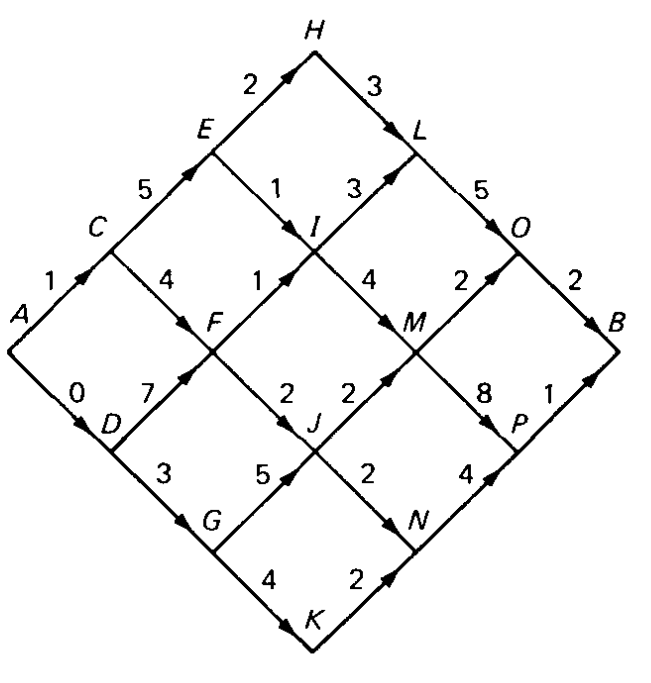
\includegraphics[width=.5\textwidth]{elem-path-problem-1}
\caption{A City Road Network (Reproduced)}
\label{fig:cityroadsrep}
\end{figure}

by using Equations[\ref{eq:fwddp1}] (Forward DP). How many additions and how many comparisons does the solution entail? How does this compare to the numbers for the original dynamic-programming solution in the text?
\end{problem}

\textbf{Solution}.

\begin{reflection}[Urge to Solve Elementary Path DP Problems with a Computer]
In a previous reflection blurb (Reflection [\ref{ref:needtoprog}]), I felt the need to create a programming framework to solve using a computer such path problems that we call ``NE--SE path problems''. 

Now the urge is stronger. We can and should solve these problems on a computer; by modeling the problem accurately, using simple data structures, and implementing algorithms correctly, these recurrences can be solved efficiently. After all, what I cannot program, I don't understand well. 

This is not going against the spirit of this book, we should solve as many problems by hand as we can, but we should not prohibit ourselves from adding a layer of personal creativity.

Another reason to implement a computer program is its indispensability when it comes to large networks. What if we are presented with a large--say, a 100-stage--network? Solving that many recurrences by hand is unthinkable. We need computer programs.

However, writing a general purpose framework for NE-SE path networks is challenging. A glance at network variants later in this book tells me that there are many `configurations' in which such a network may come. Taking care of all such tweaks is certainly not straightforward. 

Among other things, textual and programmable specifications (e.g., a complete `diamond' or a part thereof, boundary conditions, constraints) of such networks is complicated. Another need is an ability to detect, preferably quickly, an ``impossible path''. For example, there is no path from C to G or from E to N or from H to I in the network shown in Figure [\ref{fig:cityroadsrep}]. Does our DP solution detect this case, and if it does, does it say that the cost of an impossible path is $\infty$? I believe not; the DP formulation assumes that a path exists. We can and should codify certain invariants that lead to detecting impossible paths in constant time\footnote{The so-called $O(1)$ time}.

\end{reflection}

I bit the bullet and solved the problem on paper.

\begin{figure}[H]
\centering
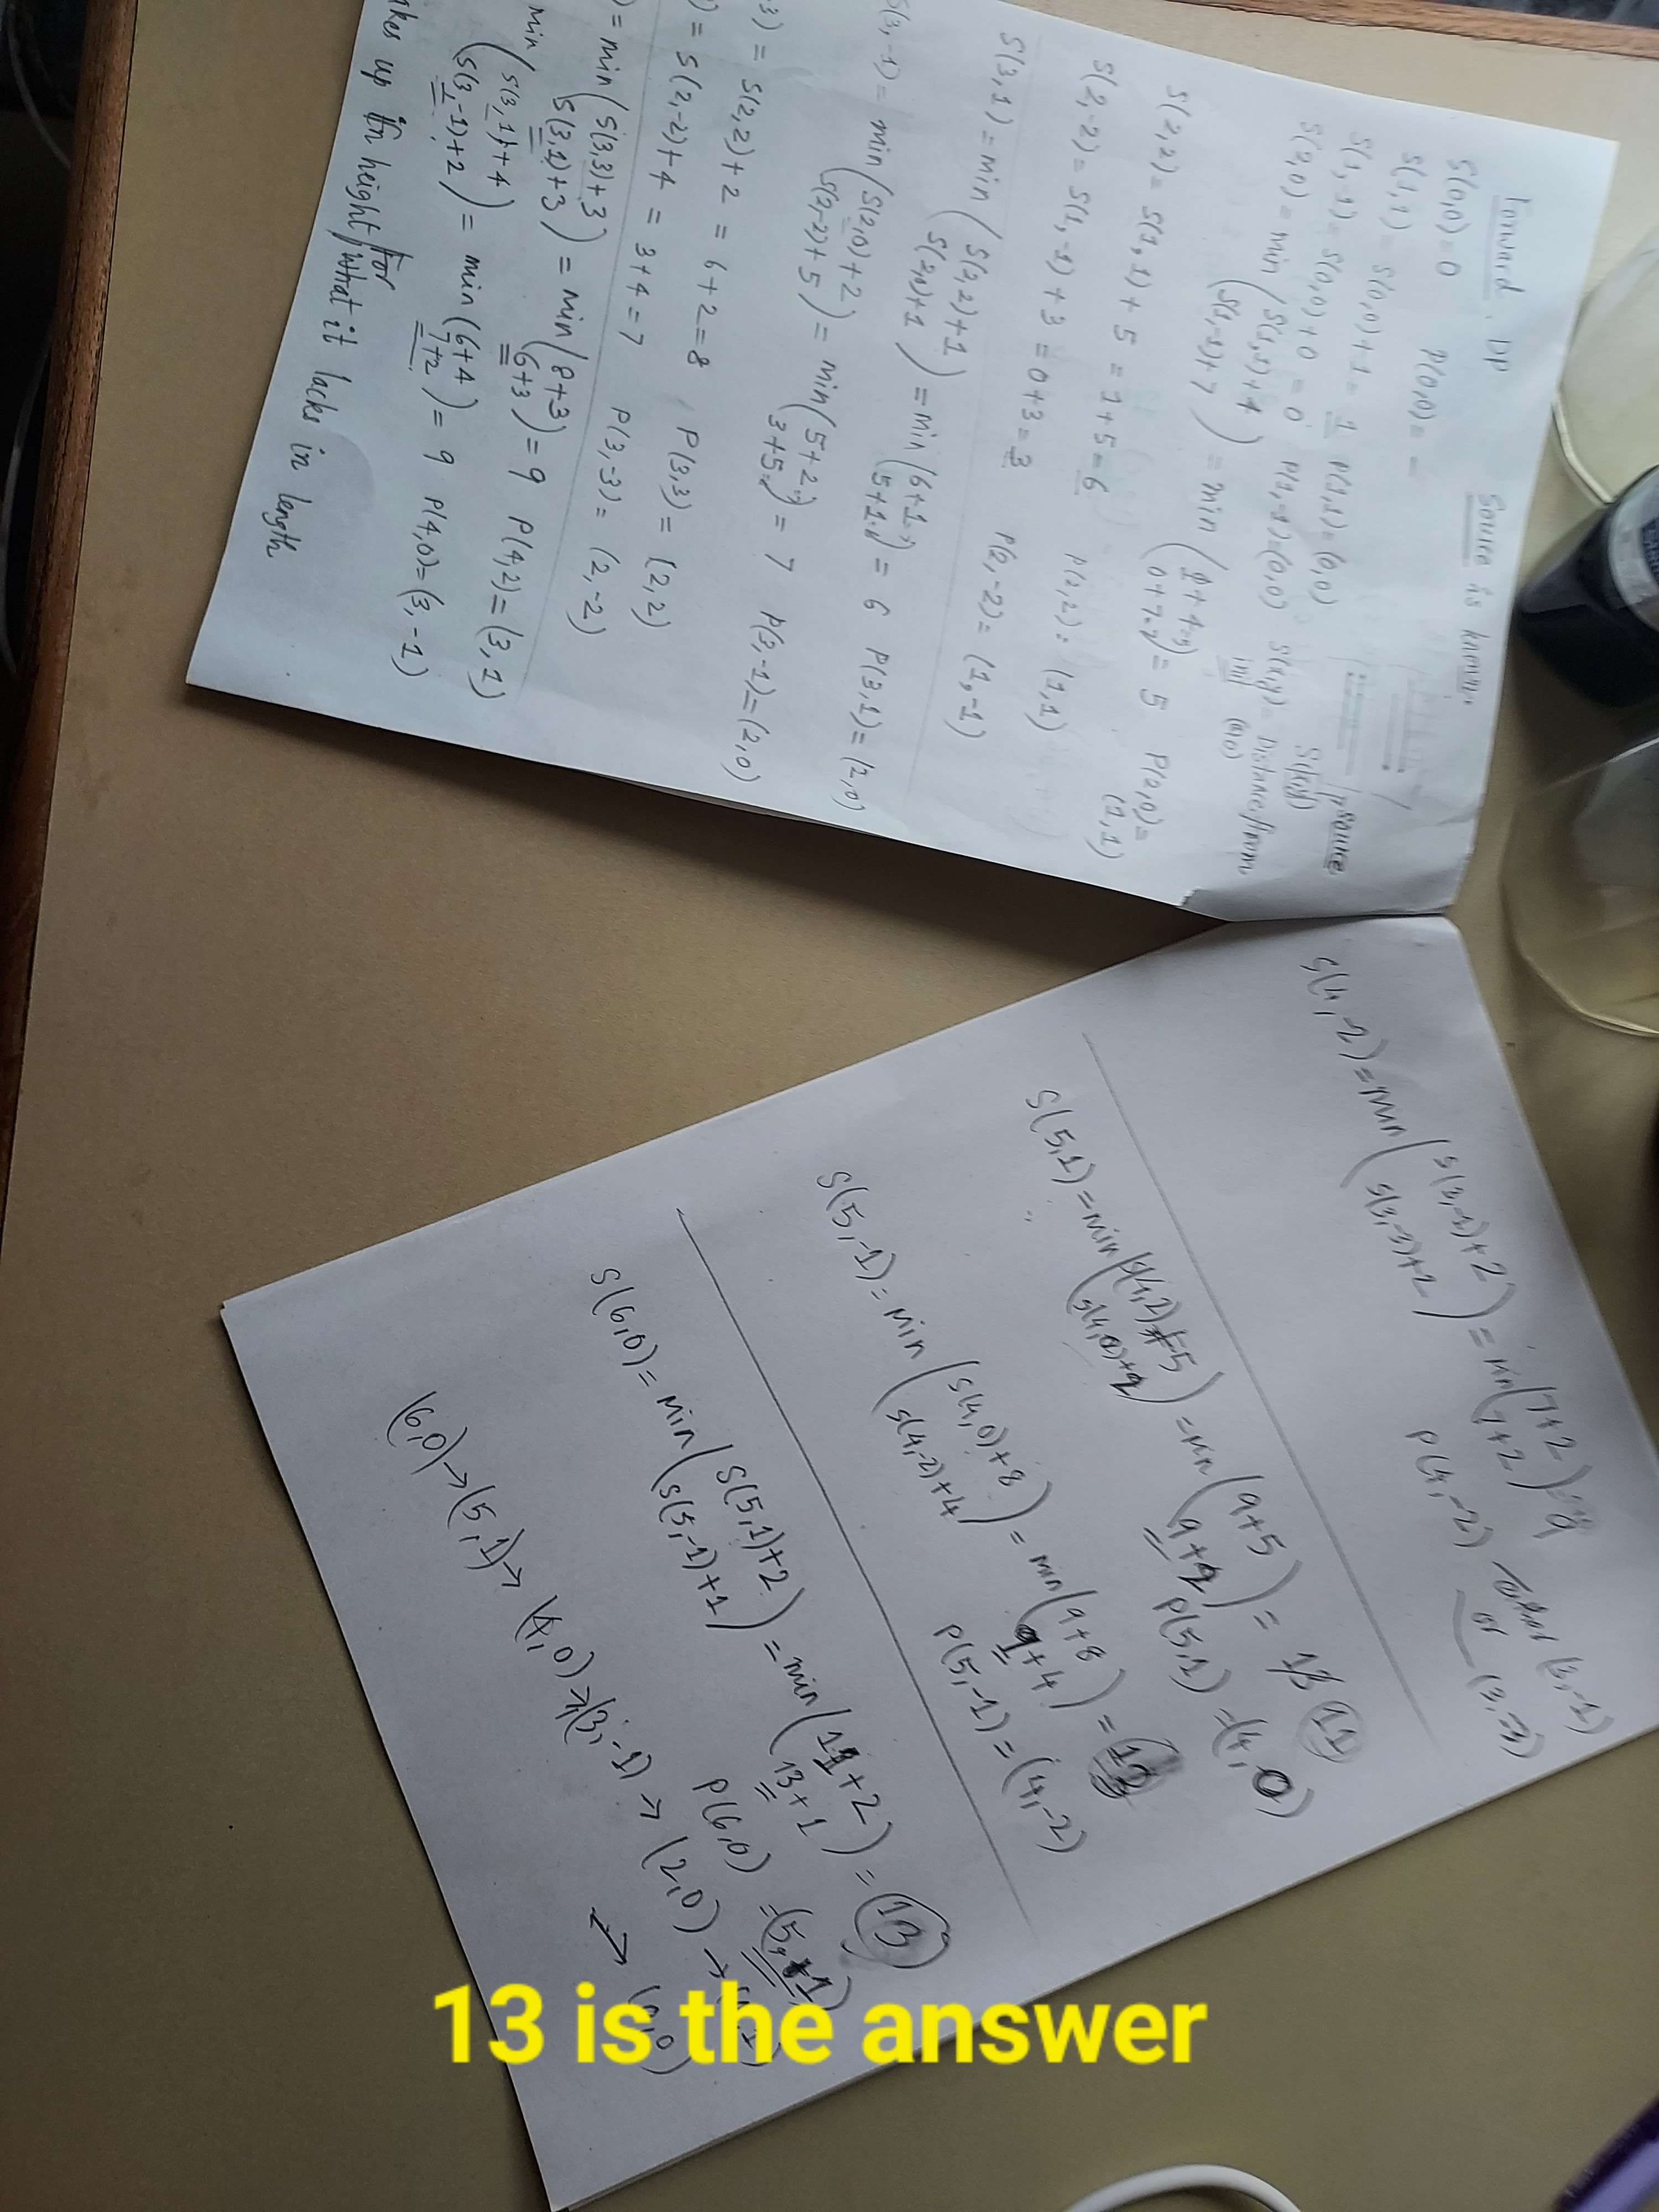
\includegraphics[width=.5\textwidth]{forward-dp-sol}
\caption{The Forward DP Formulation of Figure [\ref{fig:cityroadsrep}]}
\label{fig:forwarddpsol1}
\end{figure}

\begin{figure}[H]
\centering
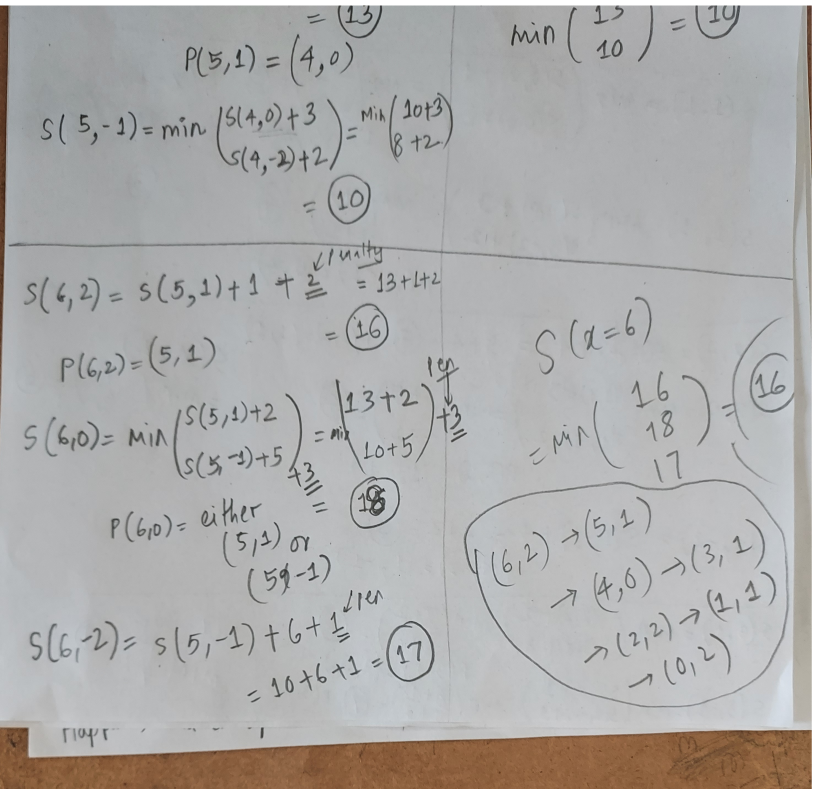
\includegraphics[width=.5\textwidth,angle=-90]{forward-dp-p1.6}
\caption{The Forward DP Formulation of Figure [\ref{fig:tbd}]}
\label{fig:forwarddpsol1}
\end{figure}

%%%-----------------------------------------------------------------------------
\MakeBibliography[nosplit]
%%%-----------------------------------------------------------------------------

%%%-----------------------------------------------------------------------------
\end{document}
%%%-----------------------------------------------------------------------------
